\subsection{Introduction}\label{subsec:introduction}
Pour représenter la relation entre un véhicule et la route d'une manière se rapprochant de la réalité, nous avons donc dû implémenter des phénomènes physiques venant des sciences de l'ingénieur. De plus, comme l'étude et la représentation d'un système  de dynamique de véhicule est une tâche plutôt difficile, nous avons décidé de procéder de manière itérative. Tout d'abord, le but était d'avoir une implémentation très basique d'un système de dynamique,  puis une fois celui-ci fonctionnel, d'itérer ce système pour intégrer des phénomènes plus délicats à implémenter, puis d'encore itérer sur ce système, etc.
Ceci nous a mené à un plan en 5 étapes.
Premièrement, implémenter les lois de Newton pour la dynamique du véhicule, puis implémenter un modèle bicycle simplifié, pour ensuite pouvoir représenter les forces sur les pneus et modéliser les glissements, et finalement pouvoir simuler les limites du pneumatique.
Nous allons maintenant vous détailler les principes physiques et l'implémentation que nous avons fournis pour chacune de ces étapes :

\subsection{Implémentation des lois de Newton pour la dynamique du véhicule}\label{subsec:implementation-des-lois-de-newton-pour-la-dynamique-du-vehicule}

Comme base de notre projet, nous avons donc commencé par implémenter la première Loi de Newton qui est le principe d'inertie, il stipule que tout corps conservera son état de repos ou de mouvement rectiligne uniforme en ligne droite dans lequel il se trouve, à moins qu'une force ne soit appliquée sur ce corps. Ainsi, un système ou corps quelconque ne peut pas se déplacer à moins qu'une force ne lui soit appliquée. Et c'est pareil pour qu'un système passe d'un état de mouvement à un état arrêté.
Dans notre implémentation, cette loi est traduite par le fait que si aucune force n'agit sur le véhicule, alors ses vitesses vont rester nulles (ou constantes si le véhicule est initialisé avec une vitesse).
Pourquoi et comment avons-nous implémenté cette loi ?
Rappelons d'abord que l'équation fondamentale de la dynamique est donnée par :
$$F = m \ .\  a$$
Avec :
\begin{itemize}
    \item $F$ la force appliquée sur le corps,
    \item $m$ la masse du corps,
    \item $a$ l'accélération résultante.
\end{itemize}

Dans notre code, nous avons appliqué cette relation en calculant les accélérations $a_x$ et $a_y$ du véhicule à partir des forces appliquées :


\begin{lstlisting}[style=CStyle,label={lst:void_computeTranslation}]
void computeTranslation(const double Fx, const double Fy, double& ax, double& ay) {
    ax = Fx / m;
    ay = Fy / m;
}
\end{lstlisting}

Ici si $F_x = 0$ et $F_y = 0$, alors $a_x$ et $a_y$, s'annulent, ce qui signifie que les vitesses restent constantes conformément au principe d'inertie.
Cependant, dès qu'on applique une force sur un objet, on génère une accélération. Cette accélération va alors modifier la vitesse de l'objet, et, comme la position est liée à la vitesse de l'objet, alors, elle évoluera dans le temps. Ce processus est décrit par des équations différentielles. Dans notre cas, nous aurons :
$$\frac{d v_x}{dt} = a_x, \quad \frac{d v_y}{dt} = a_y, \quad \frac{d r}{dt} = r_{\dot{}}$$
où $v_x$ et $v_y$ représentent les composantes de la vitesse et $r$ le lacet, l'orientation, du véhicule.

Cependant, comme notre simulateur est en temps réel, résoudre ces équations à chaque itération demanderait de nombreux cycles CPU, alors pour préserver leur usage, nous utilisons une méthode numérique, celle qui est la plus simple et efficace : la \textbf{méthode d'Euler explicite}.

Cette méthode repose sur le fait que la dérivée d'une variable $x$ notée $\dot{x}$ reste constante sur un petit intervalle de temps $dt$. Donc, on peut approximer son évolution par :
$$x(t+dt) \approx x(t) + \dot{x}(t) \times dt$$
Dans la première implémentation de notre simulateur, nous utilisons donc cette formule pour mettre à jour les vitesses et l'orientation de la voiture :
\\
\begin{itemize}
    \item \textbf{Pour la vitesse sur l'axe $x$ :}
    $$v_x(t+dt) = v_x(t)+a_x(t)\times(dt)$$
    \item \textbf{Pour la vitesse sur l'axe $y$ :}
    $$v_y(t+dt) = v_y(t)+a_y(t)\times(dt)$$
    \item \textbf{Pour l'orientation $r$ :}
    $$r(t+dt) = r(t)+\dot{r}(t)\times(dt)$$
\end{itemize}
Ici, on utilise $a_x(t)$, car c'est la dérivée de $v_x(t)$ par rapport au temps. C'est la même chose pour $a_y(t)$ qui résulte de $a_y(t)$. Ensuite, pour trouver $\dot{r}(t)$, qui est l'accélération angulaire, on applique la loi de la dynamique de rotation angulaire qui est la suivante :
$$I\dot{r}(t) = \texttt{torque}$$
où $I$ est le moment d'inertie de l'objet. En isolant $\dot{r}(t)$, on obtient :
$$\dot{r}(t)= {\frac{\texttt{torque}}{}}$$
Nous calculons cette valeur via un appel à la fonction \texttt{computeYawAcceleration(torque);} où cette relation est implémentée.

Grâce à cela, l'état de notre véhicule est mis à jour en obtenant une approximation de la solution des équations différentielles, plutôt que de les résoudre, ce qui prendrait plus de temps de calcul.
Cependant, la précision de la méthode d'Euler dépend forcément de la taille du pas qu'on lui donne ($dt$), et c'est la même chose pour des systèmes plus complexes. Dans ces cas-ci, cette méthode produira alors des erreurs significatives et la simulation deviendra instable. C'est pourquoi, plus tard dans l'implémentation de notre physique, nous avons choisi d'implémenter une méthode plus fiable dans ces cas-ci.

Ensuite pour valider le bon fonctionnement des principes physiques que nous avons décrit et implémenté nous avons réalisé une simulation de 10 secondes (avec un pas de 0,1 s), et avons utilisé \textbf{Gnuplot} pour visualiser les résultats obtenus et observer si le résultat obtenu est celui attendu. Voici la manière dont nous initialisons notre objet voiture, et indiquons la démarche à suivre pour avoir une simulation sur 10 secondes :
\begin{lstlisting}[style=CStyle,label={lst:void_simulation_etape1}]
void simulation_etape1() {
    // Initialisation du vehicule (mass=1700 kg, dist_cog_front_axle=1.5 m, dist_cog_rear_axle=1.5 m)
    OldVehicle myVehicle(1700.0, 1.5, 1.5);

    // Parametres de simulation
    double Fx = 500.0;       // Force longitudinale (N)
    double Fy = 200.0;       // Force laterale (N)
    double torque = -150.0;  // Moment de lacet (Nm)
    double dt = 0.1;         // Pas de temps (s)
    int steps = 10000;       // Simulation sur 10 secondes

    // Vecteurs pour stocker les donnees : paire (temps, valeur)
    std::vector<std::pair<double, double>>vx_data, vy_data, r_data;

    // Simulation : enregistrement des etats a chaque pas de temps
    for (int i = 0; i <= steps; ++i) {
        vx_data.push_back({t, myVehicle.vx});
        vy_data.push_back({t, myVehicle.vy});
        r_data.push_back({t, myVehicle.lacet
        myVehicle.update(dt, Fx, Fy, torque);
    }
    // ... Plot des donnees stockees dans les vecteurs avec Gnuplot

}
\end{lstlisting}

{\LARGE Question => Doit-on ajouter la partie code Gnuplot à la figure précédente ?}

Les graphiques donnés par notre implémentation donnent alors :

\begin{center}
    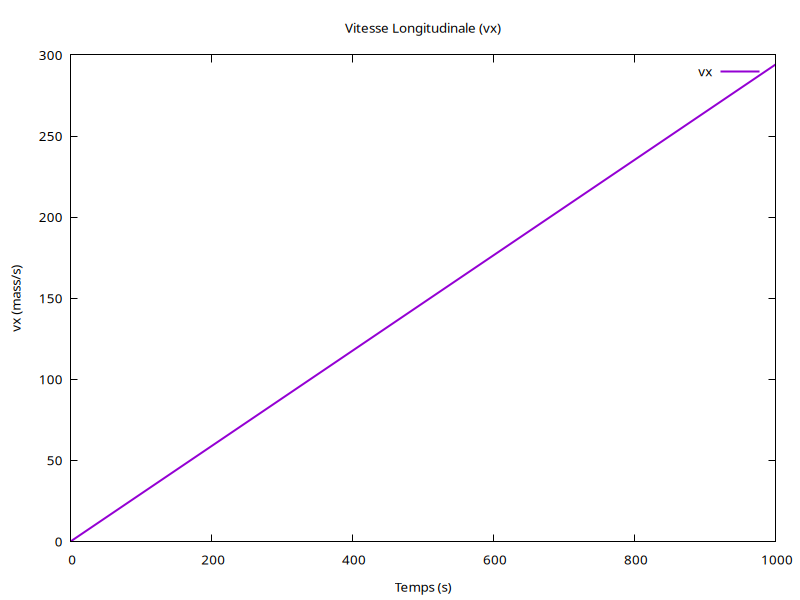
\includegraphics[width=0.70\linewidth]{Plots_Etape1/vx}
    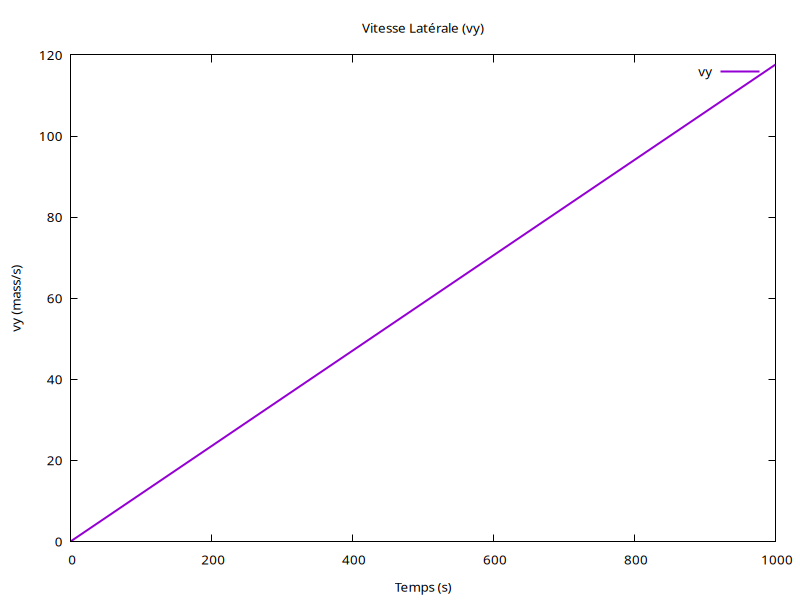
\includegraphics[width=0.70\linewidth]{Plots_Etape1/vy}
    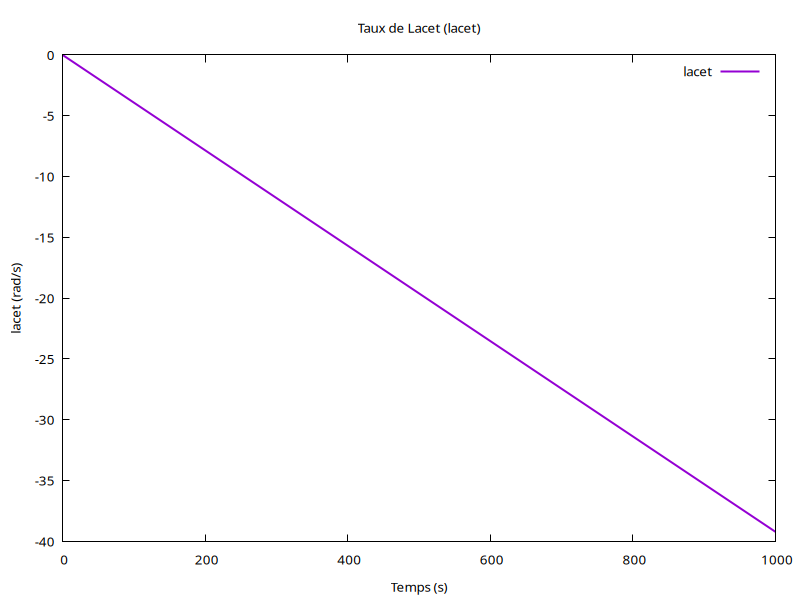
\includegraphics[width=0.70\linewidth]{Plots_Etape1/lacet}
\end{center}



\begin{itemize}
    \item \textbf{Graphique de la vitesse longitudinale ($vx$)} : Sur ce premier graphique, on observe bien que l'évolution de la vitesse sur l'axe $y$, se traduit par l'application de la force longitudinale ($ F = m \cdot a $). Et nous avons donc une accélération constante, ce qui mène à une augmentation linéaire de $vx$ au fil du temps.

    \item \textbf{Graphique de la vitesse latérale ($vy$)} : De même, le graphique représentant $vy$ permet d'observer l'effet de la force latérale appliquée.

    \item \textbf{Graphique du taux de lacet ({$\texttt{lacet}$})} : Et dernièrement, ce graphique-ci nous permet de voir l'évolution de l'orientation du véhicule. Grâce à la loi de la dynamique de rotation ($I\dot{r} = \texttt{torque}$), nous constatons que l'accélération angulaire est directement proportionnelle au couple appliqué, ce qui se traduit par une variation linéaire de $\texttt{lacet}$ au fil du temps.

\end{itemize}